\documentclass[11pt]{article}
\usepackage{geometry}
\geometry{letterpaper}
\usepackage{amssymb}
\usepackage{amsmath}
\usepackage{amsfonts}
\usepackage{graphicx}
\usepackage{setspace}
\usepackage[round]{natbib}
\bibpunct{(}{)}{;}{a}{}{;}
\textheight 20.5cm
%\topmargin -1.43cm
%\oddsidemargin 1.2cm
%\evensidemargin 1.2cm
%\textwidth 14.5cm
\usepackage{lineno}
\usepackage{xcolor}
\renewcommand\linenumberfont{\normalfont\tiny\sffamily\color{gray}}
\usepackage{booktabs}

\widowpenalty=1000
\clubpenalty=1000

\usepackage{titlesec}
\titlespacing\section{0pt}{6pt plus 4pt minus 2pt}{-8pt plus 2pt minus 2pt}
\titlespacing\subsection{0pt}{6pt plus 4pt minus 2pt}{-8pt plus 2pt minus 2pt}

%\usepackage{fontspec}
%\defaultfontfeatures{Ligatures=TeX}
%\setsansfont{Calibri}
%\setmonofont{Inconsolata}
%\usepackage{mathptmx}
%\setmainfont{Minion Pro}

% remove numbers in front of sections:
\makeatletter
\renewcommand\@seccntformat[1]{}
\makeatother

\hyphenation{meta-pop-ulation meta-pop-ulations sub-pop-ulations sub-pop-ulation e-con-o-mist en-vi-ron-men-tal pri-or-i-ti-za-tion}

\begin{document}
\raggedright

\linenumbers
\modulolinenumbers[2]
\begin{spacing}{1.6}
\setlength{\parindent}{0cm}
\section{Portfolio conservation of metapopulations under climate change}

\setlength{\parskip}{6pt} \setlength{\parindent}{0cm}

Sean C. Anderson\textsuperscript{1*}, Jonathan W. Moore\textsuperscript{1}, Trevor A. Branch?, Nicholas K. Dulvy\textsuperscript{1}, Michelle M. McClure?, Andrew B. Cooper\textsuperscript{2} (Authors and order to be discussed)

\textsuperscript{1}Department of Biological Sciences, Simon Fraser University, Burnaby BC, V5A 1S6, Canada

\textsuperscript{2}School of Resource and Environmental Management, Simon Fraser University, Burnaby, BC, V5A 1S6, Canada

\emph{Statement of authorship}: SCA, JWM, NKD, and ABC designed the analyses. SCA wrote the simulation code, analyzed the results, and wrote the first draft of the manuscript. All authors contributed substantially to revisions.

\emph{Running title}: Portfolio conservation of metapopulations (maximum 45 characters)

\emph{Keywords}: biocomplexity, Modern Portfolio Theory, portfolio effect, prioritization, resource management, range contraction, response diversity, risk assessment, salmon, stochastic simulation (maximum 10)

\emph{Type of article}: Letters

\emph{Words in abstract and main text}: (maximum 150, 5000)

\emph{Number of references}: (maximum 50)

\emph{Number of tables and figures}: 1, 5

\textsuperscript{*}Corresponding author: Sean C. Anderson; Department of Biological Sciences, Simon Fraser University, Burnaby BC, V5A 1S6; Phone: 1-778-782-3989; E-mail: sean\_anderson@sfu.ca

\setlength{\parskip}{2pt} \setlength{\parindent}{16pt}

\section{Abstract}

Managing risk is fundamental to the conservation of an endangered species. When an endangered species exists as a metapopulation, we typically manage risk at the subpopulation level. However, a portfolio approach might consider how conservation affects the ``weight'' of each population in a metapopulation ``portfolio''. Here we ask how such a portfolio approach can inform conservation priorities for metapopulations in a changing world. We develop a salmon metapopulation simulation in which population-specific productivity is driven by spatially-distributed thermal tolerance and patterns of short- and long-term environmental change. We then implement spatial conservation strategies that control subpopulation carrying capacities and evaluate the salmon portfolios along risk-return axes. We show that conserving response diversity minimizes risk given environmental stochasticity and ensures persistence given long-term environmental change. Further, conserving more subpopulations minimizes risk regardless of response diversity distribution. These findings have important implications for how we prioritize metapopulation conservation and emphasize the importance of conserving the processes that promote response diversity.

\section{Introduction}

Managing risk is fundamental to conserving endangered species \citep{burgman2005, iucn2009}. When an endangered species exists as a metapopulation, we can manage risk at two levels: at the population level or at the metapopulation level. Typically we treat sources of risk at the metapopulation level as exogenous and manage risk at the population level by manipulating hunting or fishing levels, implementing reserves, or improving connectivity \citep[e.g.][]{akcakaya2007}.

The management of financial portfolios provides another way of considering risk \citep{figge2004, koellner2006, ando2012}. Economists consider the risk and performance of a financial portfolio based on the weighting of individual investments (called assets) that make up the portfolio. Modern Portfolio Theory proposes that a set of portfolios maximizes expected return for a level of risk or minimizes risk for a level of return \citep{markowitz1952, markowitz1959}. Similarly, expected growth rate and variance of a metapopulation is a function of the variance, covariance, and size of the individual populations \citep{moore2010}. A portfolio approach to managing risk for a metapopulation might therefore consider how conservation actions affect the weight of each population in a metapopulation portfolio.

Managing Pacific salmon under the uncertainty of climate change is an ideal scenario to consider through the lens of portfolio theory for three reasons. (1) Pacific salmon form metapopulations \citep{rieman2000, schtickzelle2007} and we can consider, for example, the metapopulation in a river-catchment as a portfolio and the stream populations as assets \citep{schindler2010, moore2010}. Continuing the analogy, predators and fisheries often integrate across multiple populations \citep{hilborn2003, schindler2008}, acting as investors in the salmon portfolio. Fisheries managers and conservation agencies then act as portfolio managers by choosing which salmon habitat to prioritize for protection or restoration. (2) Many Pacific salmon metapopulations are highly threatened \citep{mcclure2003, gustafson2007, peterman2012} and will likely become more at risk as threats such as overfishing, dams, roads, logging, and particularly climate change intensify \citep[e.g.][]{lackey2003}. (3) Salmon are highly valued by society, fishers, conservation groups, and indigenous people \citep{nrc1996}. Although civil society allocates extensive resources to conserving salmonids, the scale of the problem demands a prioritization of conservation efforts \citep{allendorf1997}.

A diversified financial portfolio reduces risk by exploiting the covariance between assets --- ideally one stocks rises while another one falls --- and there are two key mechanisms that generate asynchrony in metapopulation dynamics. First, localized habitat features can filter the environment generating unique conditions for subpopulations \citep{schindler2008, rogers2008} (\emph{senu} the Moran effect). For salmon, this mechanism acts primarily during freshwater life-history stages and since many salmon species spend considerable time in the ocean \citep{quinn2005}, a second mechanism is also of key importance --- diversity of response to a shared environment \citetext{\citealp[i.e.~response diversity,][]{elmqvist2003}; \citealp[and biocomplexity][]{colwell1998}; \citealp{hilborn2003}}. This second mechanism can result from unique phenotypic or genetic traits \citep{crozier2008, kovach2012} and be derived from rapid contemporary adaption \citep{stockwell2003, fraser2011} or long-term evolution to historical conditions \citep{eliason2011}. In this paper we focus on this latter, response-diversity mechanism, and evaluate it in the context of thermal response diversity.

Salmon are strongly affected by climate warming and yet show a remarkable diversity of tolerance to temperature \citep{beacham1989, crozier2006, battin2007, crozier2008}. In addition to climate warming posing perhaps the greatest threat to global biodiversity \citep{thomas2004}, warming poses a particular threat to riverine species whose ranges are largely confined to existing habitat \citep{thomas2010} and where shallower water, compared to larger water basins, can be affected more rapidly by thermal changes \citep{isaak2010} and by snow-melt timing and extreme hydrological events \citep{crozier2008}. These consequences, and in particular warmer water itself, can combine to limit salmon productivity through, for example, oxygen limitation \citep{portner2007} leading to decreased cardiac performance \citep{eliason2011} and having profound implications for behaviour \citep{goniea2006}, disease resistance \citep{crozier2008}, and energetic costs in general \citep{rand1998}, and ultimately survival \citep{peterman1998, eliason2011}. With 29\% of Pacific Northwest salmon populations having gone extinct since Euro-American contact \citep{gustafson2007}, these populations are at risk from any further decline in fitness \citep{mcclure2003}. Yet, adverse stream temperatures are already impeding recovery of some PNW salmon populations \citep{mccullough1999}.

Here, we ask how a portfolio approach to management can inform the conservation of metapopulations in a changing world. We ask: (1) Given a plausible distribution of response diversity, how does portfolio theory inform spatial approaches to prioritizing metapopulation conservation? (2) If we don't know how response-diversity is distributed, what does portfolio theory tell us about the number of populations to conserve? To answer these questions, we develop a salmon metapopulation simulation in which spatially-distributed thermal tolerance and patterns of short- and long-term climatic change drive population-specific productivity. We then implement conservation rules of thumb that control the population-level carrying capacities and evaluate the salmon portfolios along risk and return axes, as a financial portfolio manager might. We show that conserving response diversity buffers metapopulation risk given short-term climate forcing and ensures metapopulation persistence given long-term climate warming. We then show that conserving more subpopulations buffers risk regardless of response diversity or climate trend, and conclude that considering metapopulations through portfolio theory provides a useful additional dimension through which we can consider conservation strategies.

\section{Methods}

We developed a 100-year salmon metapopulation simulation model that includes a spawner-return relationship, demographic stochasticity, straying between populations, varying responses to the environment, escapement target setting, and implementation uncertainty. Under two kinds of environmental regimes we tested different conservation rules of thumb and evaluated these plans in risk-return space similar to how financial managers evaluate financial portfolios. We illustrate the overall simulation structure in Fig.~1. We provide a package \texttt{metafolio} for the statistical software \texttt{R} \citep{r2013} as an appendix, to carry out the simulations and analyses described in this paper.

\subsection{Defining the ecological portfolio}

In our ecological portfolios, we defined assets as stream-level populations and portfolios as salmon metapopulations. We use the terms \emph{stream} and \emph{populations} interchangeably to represent the portfolio assets. We defined the portfolio investors as the stakeholders in the fishery and metapopulation performance. For example, the investors could be conservation agencies, First Nations groups, or civil society as a whole. The fisheries management agency then becomes the portfolio manager. We defined the asset value as the abundance of returning salmon in each stream and the value of the portfolio as the overall metapopulation abundance. In this scenario, the equivalent to financial rate of return is the generation-to-generation metapopulation growth rate. We defined the financial asset investment weights as the capacity of the stream populations --- specifically the unfinished equilibrium stock size --- since maintaining or restoring habitat requires money, time, and resources. Investment in a population therefore represents investing in salmon habitat conservation or restoration.

\subsection{Salmon metapopulation dynamics}

The salmon metapopulation dynamics in our simulation were governed by a spawner-return relationship with demographic stochasticity and by straying between populations.

We defined the spawner-return relationship with a Ricker model \citep{ricker1954},

\[R_{i(t)} = S_{i(t)}e^{a_{i(t)}(1-S_{i(t)}/b_i) + w_{i(t)}}\]

\noindent where $i$ represents a population, $t$ a generation time, $R$ the number of returns, $S$ the number of spawners, $a$ the productivity parameter (which can vary with the environment), and $b$ the density-dependent term (which is used as the asset weights in the portfolios). The term $w_{i(t)}$ represents first-order autocorrelated error. Formally, $w_{i(t)} = w_{ti-1} \rho_w + r_{i(t)}$, where $r_{i(t)}$ represents independent and normally distributed error with mean 0 and standard deviation of $\sigma_r$ (0.3; we include the base values in parentheses after relevant parameters). The parameter $\rho_w$ (0.4) represents the correlation between residuals from subsequent generations.

We manipulated the capacity and productivity parameters $b_i$ and $a_{i(t)}$ as part of the portfolio simulation. The capacity parameters $b_i$ were controlled by the investment weights in the populations. For example, a large investment in a stream was represented by a larger unfished equilibrium stock size $b$ for stream $i$. The productivity parameters $a_{i(t)}$ were controlled by the interaction between a temperature time series and the subpopulation thermal-tolerance curves.

We generated the thermal-tolerance performance curves according to

\[a_{i(t)} =
  \begin{cases}
    W_i (e_t - e_i^{\mathrm{opt}})^2 + a_i^{\mathrm{max}},
      & \text{if } a_{i(t)} > 0\\
      0, & \text{if } a_{i(t)} \leq 0
  \end{cases}\]

\noindent where $W_i$ controls the width of the curve for population $i$, $e_t$ represents the environmental value at generation $t$, $e_i^{\mathrm{opt}}$ represents the optimal temperature for population $i$, and $a_i^{\mathrm{max}}$ represents the maximum possible $a$ value for population $i$. We set the $W_i$ parameters (evenly spaced values increasing and decreasing between 0.05 and 0.02) and calculated the $a_i^{\mathrm{max}}$ parameters so that the area under each curve was equal (30 units). We chose parameter values such that some populations were warm-tolerant, some were cold-tolerant, and some had a wider range of thermal-tolerance, but a lower maximum productivity (see Fig.~2a). Although we refer to a thermal-tolerance curve because temperature is a dominant driver of salmonid performance \citep{mccullough1999}, our model applies to any environmental tolerance (e.g.~tolerance to stream flow volume or changes in snow melt timing \citep{crozier2008}).

We implemented straying as in \citet{cooper1999}. We arranged the subpopulations in a line and salmon were more likely to stray to streams near their natal stream. Two parameters controlled the straying: the fraction of fish $f_{\mathrm{stray}}$ (0.02) that stray from their natal stream in any generation and the rate $m$ (0.3) at which this straying between streams decays with distance. We calculated the number of salmon straying from stream $j$ to stream $i$ as

\[\mathrm{strays}_{ij(t)} = f_{\mathrm{stray}} R_{j(t)}
    \frac{e^{-m \lvert i-j \rvert }}
      {\displaystyle\sum\limits_{
        \substack{k = 1 \\ k \neq j}}^{n} 
        e^{-m \lvert k-j \rvert }}\]

\noindent where $R_{j(t)}$ is the number of returning salmon at generation $t$ whose natal stream was stream $j$. The subscript $k$ represents a stream ID and $n$ the number of populations. The denominator is a normalizing constant to ensure the desired fraction of fish stray. See Figure \ref{f:stray} for an example straying matrix.

Our simulation did not account for the homogenization of diversity due to straying. For example, all salmon in population A maintained the same thermal-tolerance curve regardless of how many salmon it received from population B. However, the low straying rates in our simulation rate should render this effect minimal except for populations at low abundance. In our model, the main implication is that, in reality, populations that reach a low abundance may reach demographic extinction, potentially suffer consequences such as inbreeding depression \citep{wang2002} and subsequently contribute little to response diversity.

\subsection{Fishing}

Our simulation used a simple set of rules to establish escapement targets and harvest the fish. Every five years our simulation fitted a spawner-return function and the target harvest rate $H_{\mathrm{tar}}$ was set based on \citet{hilborn1992} as

\[H_{\mathrm{tar}} = \frac{A}{b (0.5 - 0.07a)}
  \label{eq:esc}\]

\noindent where $A$ represents the return abundance and $a$ and $b$ represent the Ricker model parameters. We included implementation uncertainty in the actual harvest rate $H_{\mathrm{act}}$ as

\[H_{\mathrm{act}} = \mathrm{beta}(\alpha_h, \beta_h)\]

\noindent where $\alpha_h$ and $\beta_h$ are the location and shape parameters in a beta distribution. They can be calculated from the desired mean $H_{\mathrm{tar}}$ and standard deviation $\sigma_h$ (0.05) as \citep[p.~97]{morgan1990}

\[\begin{aligned}
  \alpha_h &= H_{\mathrm{tar}}^2
                \left(
                \frac{1 - H_{\mathrm{tar}}}{\sigma_h^2} - \frac{1}{H_{\mathrm{tar}}}
                \right)\\
   \beta_h &= \alpha \left({\frac{1}{H_{\mathrm{tar}}} - 1}\right).\end{aligned}\]

\noindent Further, to establish a range of spawner-return values and to mimic the start of an open-access fishery, for the first 30 years we drew the fraction of fish harvested randomly from a uniform distribution between 0.1 and 0.9. We discarded these initial 30 years as a burn-in period.

\subsection{Environmental dynamics}

Environmental dynamics typically have both short- and long-term fluctuations. We evaluated portfolio performance under these two components separately. We represented short-term dynamics as a stationary first-order autoregressive process, AR(1), with correlation $\rho_e$ (0.1)

\[e_t = e_{t-1} \rho_e + d_t, d_t \sim \mathrm{N}(0, \sigma_d)\]

\noindent where $e_t$ represents the environmental value in generation $t$ and $d$ represents normally distributed deviations of mean 0 and standard deviation $\sigma_d$ (2). We represented long-term environmental dynamics as a linear shift in the environmental value through time

\[e_t = \beta_e t - \overline{\beta_e t}\]

\noindent where $\beta_e$ (0.114) represents the slope. To maintain a balanced response, we centered the trend by subtracting the mean $\overline{\beta_e t}$ so that midway through the simulation (after any burn-in period) the environmental value was at the mean environmental tolerance.

Combining salmon population dynamics, fishing, and environmental dynamics, we illustrate the components of an example simulation in Fig.~3.

\subsection{Conservation rules of thumb}

We evaluated two sets of conservation rules of thumb: (1) strategies to conserve spatial response diversity, and (2) a scenario where we know little about response diversity and we're left with a choice of how many populations to conserve.

We evaluated four spatial conservation rules of thumb (Fig.~2b--e). In all spatial scenarios, we conserved four populations and set the unfished equilibrium biomass of the remaining populations to near elimination (five salmon). These reduced populations could still receive straying salmon but were unlikely to rebuild on their own to a substantial abundance. The four scenarios we considered were:

\begin{enumerate}
\def\labelenumi{\arabic{enumi}.}
\itemsep1pt\parskip0pt\parsep0pt
\item
  Conserve an even sampling of response diversity.
\item
  Conserve the middle section of the metapopulation (conserve stable populations).
\item
  Conserve the lower half of the metapopulation (conserve cool-tolerant populations).
\item
  Conserve the upper half of the metapopulation (conserve warm-tolerant populations).
\end{enumerate}

In reality we rarely know precise levels of response diversity. We therefore considered a case where the conservation was randomly assigned with respect to response diversity but where different numbers of streams could be conserved. We considered conserving from two to 16 streams. Similarly to the spatial strategies, we reduced the capacity of the remaining streams to the nominal level of five salmon.

\section{Results}

\subsection{Which populations to conserve?}

\emph{Given short-term environmental fluctuations}, conserving response diversity buffers the risk properties of an ecological portfolio (Fig.~4a). In our model, the median variance of metapopulation growth rate was X times lower given balanced response diversity (full range of responses or most stable only vs.~conserving one half or the other). This increase in stability occurred despite the portfolio being comprised of warm and cool-thriving populations that were more variable on their own than populations with wide thermal-tolerance curves. We can see the mechanism behind these portfolio properties by inspecting example population time series (Fig.~4c, d). If only the upper or lower half of response diversity is conserved, the portfolio tends to alternate between performing well and poorly depending on the environmental conditions resulting in a risker portfolio (Fig.~4e). This risk is buffered with balanced response diversity (Fig.~4c).

\emph{Given long-term environmental change}, the choice of which populations to conserve affects the ``return'' (metapopulation growth rate) properties of an ecological portfolio (Fig.~4b). By conserving balanced response diversity, an ecological manager is hedging his or her bets on the environmental trend and how the populations will respond. The typical metapopulation growth rate for a balanced response diversity strategy was zero --- the metapopulation neither increased or decreased in abundance in the long run. The example metapopulation abundance time series (Fig.~4d, f) illustrate the mechanism. By conserving response diversity, when one population is doing poorly, another is doing well and the metapopulation abundance remains stationary through time. If a manager had invested in the populations that were doing well at the beginning they would have had the lowest rate-of-return portfolio in the end (purple portfolios in Fig.~4f).

\subsection{How many populations to conserve?}

In a scenario where we don't know the distribution of population-level response diversity, portfolio optimization informs us that investing in more populations buffers portfolio risk regardless of environmental trend (Fig.~5).

\emph{Given short-term environmental fluctuations}, conserving more populations buffers portfolio risk (Fig.~5a), and at the same time, the random conservation of response diversity creates a spread of metapopulation risk for the same number of populations conserved. For example, a metapopulation with eight conserved populations is X times less risky than a metapopulation with only four. We can see this risk-buffering effect through example metapopulations in Fig.~5c and 5d. We note that the risk-return axes of portfolio optimization ignore the absolute-abundance dimension (Fig.~5d) --- as one would expect, conserving fewer populations also results in lower-abundance metapopulations.

\emph{Given long-term environmental change}, conserving more populations also buffers portfolio risk. However, in contrast to the short-term environmental noise scenario, the unknown response diversity creates a spread of possible metapopulation return for the same number of conserved populations (Fig.~5b). Here, the number of populations conserved buffers non-systematic (primarily demographic) stochasticity.

\section{Discussion}

Our model demonstrates how population diversity can stabilize realistic metapopulations under climate change. We show how maintaining populations with a variety of thermal-tolerances reduces risk caused by short-term environmental stochasticity and optimizes chances for long-term persistence given climate change. Further, without knowing how response diversity is distributed, conserving more subpopulations reduces metapopulation risk regardless of environmental trend and response-diversity distribution. Combined, these two findings illustrate that focusing on well-performing stocks now at the detriment of others is at best equivalent to a risky but efficient portfolio, and at worst a poorly-performing risky portfolio. In this discussion, we begin by linking our model with real-world conservation issues for Pacific Northwest salmon and considering the implications of our results for salmon conservation and management. We then consider broader research priorities and extensions that our results suggest for metapopulation conservation.

The primary finding from our simulation model is the importance of response diversity in buffering risk and ensuring long-term persistence in the face of environmental uncertainty. Thus, our results emphasize the need to make the maintenance of response diversity, and the processes that promote response diversity, a primary goal of conservation and recovery efforts \citep{moore2010}. For example, since habitat heterogeneity can lead to local adaptation \citep{taylor1991, fraser2011}, our results emphasize the need to maintain a diversity of salmon habitat \citep{rogers2008}. Our results can also inform habitat prioritization decisions. If conservation actions must be prioritized, then our model suggests we should focus on populations that aren't spatially contiguous, as long as sufficient straying is maintained, to maximize diversity of response to the environment. Finally, our results demonstrate the advantages of avoiding structures that artificially remove response diversity. For salmon, dams are a prominent example \citep{waples2007, pess2012}. Dams can have a double impact whereby their introduction selectively eliminates a large swath of contiguous habitat, perhaps analogous to our upper- or lower-half scenarios in Fig.~4, and then mitigation approaches such as hatcheries can further reduce population and response diversity if not carefully managed \citep{waples1991a, mobrand2005}.

Our simulation model emphasizes the importance of thinking at the portfolio level --- considering aggregate risk and performance for ecological portfolios. Although our results may appear intuitive, we often don't often consider aggregate risk and only by simultaneously considering aggregate risk and return can we optimally diversify ecological systems \citep{ando2012}. Thus we can think of portfolio risk-return performance as another dimension of conservation. This dimension emphasizes the value of a broader scale of management and focussing not just on currently productive populations but also on less productive populations to reduce long-term aggregate risk \citep[e.g.][]{hilborn2003, price2008}. This perspective does not negate an understanding at a finer scale, say of individual fish stocks. Rather, as in finance, it requires both an understanding of stock performance and an assessment of their covariance to predict properties of the portfolio as a whole.

THE FOLLOWING PARAGRAPH IS STILL BEING PIECED TOGETHER

Our findings support the existence of and inform the implementation of a number of existing guidelines and management structures for PNW salmonids. In the US, Evolutionarily Significant Units (ESUs) represent salmon populations that are reproductively isolated with an evolutionary heritage \citep{waples1991, moritz1994} and finer-scale Viable Salmonid Populations (VSPs) represent groups of fish that spawn in a given lake or stream in a particular season \citep{mceacheran2000}. In Canada, the rough equivalent to the ESU is a Conservation Unit (CU) as defined in the Wild Salmon Policy \citep{dfo2005wsp}. A CU consists of a group of salmon that are reproductively isolated and that if lost would be unlikely to recolonize in a reasonable time frame \citep{dfo2005wsp}. Both the US and Canadian guidelines recognize still-finer-scale population structure. We suggest that a salmon portfolio in our model could represent an ESU or CU and that the lessons learned from our models are thus directly applicable to management guidelines in the PNW.

VSP guidelines \citep{mceacheran2000} suggest\ldots{}

\begin{itemize}
\item
  maintaining diversity of a variety of forms to buffer against short-term environmental changes and adaptation to long-term environmental changes
\item
  conservation efforts should not focus exclusively where there is currently an abundance of salmon
\item
  metapopulation (multiple populations with some exchange) are important to maintain
\item
  some should be close for straying, but some should be far apart to reduce risk from sudden environmental change
\item
  important to incorporate uncertainty of ESU-level processes into assessments
\end{itemize}

CU guidelines \citep{dfo2005wsp} suggest\ldots{}

-

Our recommendations support a number of VSP and CU guidelines. For example, VSP guidelines suggest\ldots{} and the first objective of CU\ldots{} Therefore, we suggest an ESU or CU could represent a salmon portfolios and the lessons learned from models such as ours are directly applicable to management guidelines in the PNW.

END IN PROGRESS TEXT

Our model is unique in that it is the first to consider risk for metapopulations as a whole while identifying the role of response diversity in buffering risk. Our model follows from the work of \citet{cooper1999} who showed the importance of metapopulation habitat structure for salmonid conservation and \citet{moore2010} who linked salmon portfolio performance to asynchrony in population dynamics. Our model complements existing simulation-based salmon-habitat prioritization models that emphasize detailed assessment of individual stocks and we compare two of them here. One a frequently used simulation-based habitat-prioritization model, the Shiraz model \citep{scheuerell2006}, focuses on detailed conditioning of the habitat-population-dynamics relationship for a single salmon population. While the Shiraz model can be applied to an entire watershed it combines the populations together as a single unit. In contrast to our model, the Shiraz model breaks the spawner-recruit model into multiple stages. A second prioritization scheme proposes using population viability analysis (PVA) or surrogate measures of population viability combined with an assessment of the genetic consequences of losing various populations \citep{allendorf1997}. \citet{allendorf1997}, however, also focus on the assessment of individual stocks without considering their covariance and therefore the performance of the salmon portfolio as a whole. Compared to these detailed population-specific models, our model is at this stage primarily conceptual, but could be conditioned on real systems or expanded to incorporate greater life-stage realism. Our intention was to develop a parsimonious model to explore the salient aspects of metapopulation-portfolio performance.

We suggest a number of specific extensions to our simulation model. First our model could be extended beyond thermal response diversity. For salmon this might include response diversity to interdecadal climate signals such as the Pacific Decadal Oscillation \citep{mantua2002}, or to stream flow and dissolved oxygen \citep{priede1988}. Second, our model could be extended to metapopulations of other taxa, to ecological communities (after accounting for species interactions), or to meta-communities. Third, an extension of our model would consider the Moran or environmental-filter concept \citep{schindler2008, rogers2008} where populations experience increasingly different environmental forces at further distances. Fourth, a model could consider the contribution of contemporary evolution \citep{stockwell2003}. This rapid adaptation to changes in the environment could strongly affect portfolio performance and emphasizes the importance of maintaining genetic diversity. Finally, our model could be conditioned on a system of interest --- a particular river basin for example --- and the management metapopulation portfolio could be optimized across conservation and restoration options as part of a formal decision analysis.

Our results suggest three broad research priorities. First, our work highlights the importance of research that identifies response diversity \citep[e.g.][]{eliason2011}, spatial asynchrony \citep[e.g.][]{thorson2013}, and in particular the management schemes that promote these processes \citep{moore2010}. Our work highlights how these processes can contribute to reducing risk and increasing the likelihood of metapopulation persistence given environmental uncertainty. Second, our work suggests the importance of identifying the drivers of productivity across populations and environmental scenarios. For example, what is the relative effect on productivity of population density, an environment-recruitment relationship, and environmental regime shifts, and what management approaches are robust to our uncertainty about these contributions \citep{vert-pre2013}? Third, our work suggests research that identifies real-life case studies as in situ experiments testing our conclusions. The question remains, does managing metapopulation portfolios using Modern Portfolio Theory result in better outcomes that are in line with the societal goals?

In conclusion, our results demonstrate the utility of considering metapopulations in a portfolio context and the power of portfolio simulation to consider robust management strategies that minimize metapopulation risk and maximize growth under uncertain environmental conditions. Our findings show that response diversity buffers metapopulation risk given short-term environmental stochasticity and ensures persistence given longterm regime changes. Further, our findings show that, independent of response-diversity, conserving more populations buffers metapopulation risk. These results point to the critical importance of choosing management, conservation, and restoration actions that preserve and promote response diversity and are robust to our uncertainty about response diversity distribution and future climatic conditions.

\section{Acknowledgements}

Funding was provided by NSERC (ABC, NKD, SCA), the Canada Research Chairs Program (NKD), Simon Fraser University, the Liber Ero Chair of Coastal Science and Management (JWM), Fulbright Canada (SCA), and a Garfield Weston Foundation/B.C. Packers Ltd. Graduate Fellowship in Marine Sciences (SCA).

\bibliographystyle{ecologyletters2}

\bibliography{jshort,ms}

\clearpage

\section{Figures}

\setlength{\parskip}{6pt} \setlength{\parindent}{0cm} \includegraphics[height=5.5in]{../examples/simulation-diagram3.pdf}

Fig.~1: Flow chart of the salmon-metapopulation simulation. There are $n$ salmon populations and $t$ generations. Blue text indicates values that are generated before the simulation progresses through time. Red text indicates steps in which calculations are performed through time. Black text indicates values that are calculated. Grey text indicates parameters that can be set. Green text indicates the looping structure of the simulation.

\clearpage
\includegraphics[width=3.0in]{../examples/thermal-curve-scenarios.pdf}

Fig.~2: Different ways of prioritizing response-diversity conservation. Panel a shows thermal tolerance cures for ten possible populations and panels b--e show different ways of prioritizing four of those populations. The curves describe how productivity varies with temperature for a given population. Some populations thrive at low temperatures (cool colours) and some at warm temperatures (warm colours). Some are tolerant to a wider range of environmental conditions (yellow-to-green colours) but with a lower maximum productivity. The total possible productivity (the area under the curves) is the same for each population.

\clearpage
\includegraphics[width=4.0in]{../examples/spatial-arma-sim.pdf}

Fig.~3: The components of an example metapopulation simulation. We show, from top to bottom, the environmental signal, the resulting productivity parameter (Ricker $a$), the salmon returns, fisheries catch, salmon escapement, salmon straying from their natal streams, salmon joining from other streams, spawner-return residuals on a log scale, and the estimated $a$ and $b$ parameters in the fitted Ricker curve. The colored lines indicate populations that thrive at low (cool colours) to high (warm colours) temperatures.

\clearpage
\includegraphics[width=5.0in]{../examples/spatial-mv.pdf}

Fig.~4: The importance of preserving environmental response diversity through spatial conservation strategies. The conservation strategies correspond to Fig.~2 and represent conserving a range of responses (green), the most stable populations only (orange), or one type of environmental response (purple and pink). In risk-return space we show environmental scenarios that are comprised primarily of (a) short-term and (b) long-term environmental fluctuations. The dots show simulated metapopulations and the contours show 25\% and 75\% quantiles across 500 simulations per strategy. We also show example metapopulation abundance time series for the (c, e) short-term and (d, f) long-term environmental-fluctuation scenarios.

\clearpage
\includegraphics[width=5.0in]{../examples/cons-plans-n.pdf}

Fig.~5: The importance of preserving as many subpopulations as possible when we don't know how response diversity is distributed. In risk-return space we show environmental scenarios that are comprised primarily of (a) short-term and (b) long-term environmental fluctuations. We show metapopulations in which 2 (red), 4 (orange), 8 (yellow), or 16 (green) populations of random response diversity are conserved. The dots show simulated metapopulations and the contours show 25\% and 75\% quantiles across 500 simulations per strategy. We also show example metapopulation (c) rate-of-change and (d) abundance time series for the short-term environmental-fluctuation scenario.


\bibliographystyle{ecologyletters2}
%\bibliography{jshort,ms}

\begin{thebibliography}{50}
\expandafter\ifx\csname natexlab\endcsname\relax\def\natexlab#1{#1}\fi
\expandafter\ifx\csname url\endcsname\relax
  \def\url#1{\texttt{#1}}\fi
\expandafter\ifx\csname urlprefix\endcsname\relax\def\urlprefix{URL }\fi

\bibitem[{Allendorf \emph{et~al.}(1997)Allendorf, Bayles, Bottom, Currens,
  Frissell, Hankin, Lichatowich, Nehlsen, Trotter \& Williams}]{allendorf1997}
1.\\
Allendorf, F.~W., Bayles, D., Bottom, D.~L., Currens, K.~P., Frissell, C.~A.,
  Hankin, D., Lichatowich, J.~A., Nehlsen, W., Trotter, P.~C. \& Williams,
  T.~H. (1997).
\newblock Prioritizing {Pacific} salmon stocks for conservation.
\newblock \emph{Conserv. Biol.}, 11, 140--152.

\bibitem[{Anderson \emph{et~al.}(2013)Anderson, Cooper \& Dulvy}]{anderson2013}
2.\\
Anderson, S.~C., Cooper, A.~B. \& Dulvy, N.~K. (2013).
\newblock Ecological prophets: Quantifying metapopulation portfolio effects.
\newblock \emph{Methods Ecol. Evol.}, 4, 971--981.

\bibitem[{Ando \& Mallory(2012)}]{ando2012}
3.\\
Ando, A.~W. \& Mallory, M.~L. (2012).
\newblock Optimal portfolio design to reduce climate-related conservation
  uncertainty in the {Prairie Pothole Region}.
\newblock \emph{Proc. Natl. Acad. Sci. U.S.A.}, 109, 6484--6489.

\bibitem[{Balvanera \emph{et~al.}(2006)Balvanera, Pfisterer, Buchmann, He,
  Nakashizuka, Raffaelli \& Schmid}]{balvanera2006}
4.\\
Balvanera, P., Pfisterer, A.~B., Buchmann, N., He, J.-S., Nakashizuka, T.,
  Raffaelli, D. \& Schmid, B. (2006).
\newblock Quantifying the evidence for biodiversity effects on ecosystem
  functioning and services.
\newblock \emph{Ecol. Lett.}, 9, 1146--1156.

\bibitem[{Battin \emph{et~al.}(2007)Battin, Wiley, Ruckelshaus, Palmer, Korb,
  Bartz \& Imaki}]{battin2007}
5.\\
Battin, J., Wiley, M.~W., Ruckelshaus, M.~H., Palmer, R.~N., Korb, E., Bartz,
  K.~K. \& Imaki, H. (2007).
\newblock Projected impacts of climate change on salmon habitat restoration.
\newblock \emph{Proc. Natl. Acad. Sci. U.S.A.}, 104, 6720--6725.

\bibitem[{Beechie \emph{et~al.}(2013)Beechie, Imaki, Greene, Wade, Wu, Pess,
  Roni, Kimball, Stanford, Kiffney \& Mantua}]{beechie2013}
6.\\
Beechie, T., Imaki, H., Greene, J., Wade, A., Wu, H., Pess, G., Roni, P.,
  Kimball, J., Stanford, J., Kiffney, P. \& Mantua, N. (2013).
\newblock Restoring salmon habitat for a changing climate.
\newblock \emph{River Res. Applic.}, 29, 939--960.

\bibitem[{Cooper \& Mangel(1999)}]{cooper1999}
7.\\
Cooper, A.~B. \& Mangel, M. (1999).
\newblock The dangers of ignoring metapopulation structure for the conservation
  of salmonids.
\newblock \emph{Fish. Bull.}, 97, 213--226.

\bibitem[{Crozier \emph{et~al.}(2008)Crozier, Hendry, Lawson, Quinn, Mantua,
  Battin, Shaw \& Huey}]{crozier2008}
8.\\
Crozier, L.~G., Hendry, A.~P., Lawson, P.~W., Quinn, T., Mantua, N.~J., Battin,
  J., Shaw, R.~G. \& Huey, R.~B. (2008).
\newblock Potential responses to climate change in organisms with complex life
  histories: evolution and plasticity in {Pacific} salmon.
\newblock \emph{Evol. Appl.}, 1, 252--270.

\bibitem[{de~Mazancourt \emph{et~al.}(2013)de~Mazancourt, Isbell, Larocque,
  Berendse, De~Luca, Grace, Haegeman, Wayne~Polley, Roscher, Schmid, Tilman,
  van Ruijven, Weigelt, Wilsey \& Loreau}]{demazancourt2013}
9.\\
de~Mazancourt, C., Isbell, F., Larocque, A., Berendse, F., De~Luca, E., Grace,
  J.~B., Haegeman, B., Wayne~Polley, H., Roscher, C., Schmid, B., Tilman, D.,
  van Ruijven, J., Weigelt, A., Wilsey, B.~J. \& Loreau, M. (2013).
\newblock Predicting ecosystem stability from community composition and
  biodiversity.
\newblock \emph{Ecol. Lett.}, 16, 617--625.

\bibitem[{DFO(2005)}]{dfo2005wsp}
10.\\
DFO (2005).
\newblock Canada's policy for conservation of wild {Pacific} salmon.
\newblock Tech. rep., Fisheries and Oceans Canada, Vancouver, BC.

\bibitem[{Eliason \emph{et~al.}(2011)Eliason, Clark, Hague, Hanson, Gallagher,
  Jeffries, Gale, Patterson, Hinch \& Farrell}]{eliason2011}
11.\\
Eliason, E.~J., Clark, T.~D., Hague, M.~J., Hanson, L.~M., Gallagher, Z.~S.,
  Jeffries, K.~M., Gale, M.~K., Patterson, D.~A., Hinch, S.~G. \& Farrell,
  A.~P. (2011).
\newblock Differences in thermal tolerance among sockeye salmon populations.
\newblock \emph{Science}, 332, 109--112.

\bibitem[{Elmqvist \emph{et~al.}(2003)Elmqvist, Folke, Nystr{\"o}m, Peterson,
  Bengtsson, Walker \& Norberg}]{elmqvist2003}
12.\\
Elmqvist, T., Folke, C., Nystr{\"o}m, M., Peterson, G., Bengtsson, J., Walker,
  B. \& Norberg, J. (2003).
\newblock Response diversity, ecosystem change, and resilience.
\newblock \emph{Front. Ecol. Environ.}, 1, 488--494.

\bibitem[{Figge(2004)}]{figge2004}
13.\\
Figge, F. (2004).
\newblock Bio-folio: applying portfolio theory to biodiversity.
\newblock \emph{Biodivers. Conserv.}, 13, 827--849.

\bibitem[{Fraser \emph{et~al.}(2011)Fraser, Weir, Bernatchez, Hansen \&
  Taylor}]{fraser2011}
14.\\
Fraser, D.~J., Weir, L.~K., Bernatchez, L., Hansen, M.~M. \& Taylor, E.~B.
  (2011).
\newblock Extent and scale of local adaptation in salmonid fishes: review and
  meta-analysis.
\newblock \emph{Heredity}, 106, 404--420.

\bibitem[{Gustafson \emph{et~al.}(2007)Gustafson, Waples, Myers, Weitkamp,
  Bryant, Johnson \& Hard}]{gustafson2007}
15.\\
Gustafson, R.~G., Waples, R.~S., Myers, J.~M., Weitkamp, L.~A., Bryant, G.~J.,
  Johnson, O.~W. \& Hard, J.~J. (2007).
\newblock Pacific salmon extinctions: quantifying lost and remaining diversity.
\newblock \emph{Conserv. Biol.}, 21, 1009--1020.

\bibitem[{Haak \& Williams(2012)}]{haak2012}
16.\\
Haak, A.~L. \& Williams, J.~E. (2012).
\newblock Spreading the risk: native trout management in a warmer and
  less-certain future.
\newblock \emph{N. Am. J. Fish. Manage.}, 32, 387--401.

\bibitem[{Hannah \emph{et~al.}(2002)Hannah, Midgley, Lovejoy, Bond, Bush,
  Lovett, Scott \& Woodward}]{hannah2002a}
17.\\
Hannah, L., Midgley, G.~F., Lovejoy, T., Bond, W.~J., Bush, M., Lovett, J.~C.,
  Scott, D. \& Woodward, F.~I. (2002).
\newblock Conservation of biodiversity in a changing climate.
\newblock \emph{Conserv. Biol.}, 16, 264--268.

\bibitem[{Hilborn \emph{et~al.}(2003)Hilborn, Quinn, Schindler \&
  Rogers}]{hilborn2003}
18.\\
Hilborn, R.~W., Quinn, T., Schindler, D. \& Rogers, D. (2003).
\newblock Biocomplexity and fisheries sustainability.
\newblock \emph{Proc. Natl. Acad. Sci. U.S.A.}, 100, 6564--6568.

\bibitem[{Hilborn \& Walters(1992)}]{hilborn1992}
19.\\
Hilborn, R.~W. \& Walters, C. (1992).
\newblock \emph{Quantitative Fisheries Stock Assessment: Choice, Dynamics, and
  Uncertainty}.
\newblock Chapman and Hall, London.

\bibitem[{Ives \& Carpenter(2007)}]{ives2007}
20.\\
Ives, A.~R. \& Carpenter, S.~R. (2007).
\newblock Stability and diversity of ecosystems.
\newblock \emph{Science}, 317, 58--62.

\bibitem[{Johnson \& Schindler(2013)}]{johnson2013a}
21.\\
Johnson, S.~P. \& Schindler, D.~E. (2013).
\newblock Marine trophic diversity in an anadromous fish is linked to its
  life-history variation in fresh water.
\newblock \emph{Biol. Lett.}, 9, 20120824.

\bibitem[{Koellner \& Schmitz(2006)}]{koellner2006}
22.\\
Koellner, T. \& Schmitz, O.~J. (2006).
\newblock Biodiversity, ecosystem function, and investment risk.
\newblock \emph{BioScience}, 56, 977--985.

\bibitem[{Lackey(2003)}]{lackey2003}
23.\\
Lackey, R.~T. (2003).
\newblock {Pacific Northwest} salmon: Forecasting their status in 2100.
\newblock \emph{Rev. Fish. Sci.}, 11, 35--88.

\bibitem[{Margules \& Pressey(2000)}]{margules2000}
24.\\
Margules, C.~R. \& Pressey, R.~L. (2000).
\newblock Systematic conservation planning.
\newblock \emph{Nature}, 405, 243--253.

\bibitem[{Markowitz(1952)}]{markowitz1952}
25.\\
Markowitz, H. (1952).
\newblock Portfolio selection.
\newblock \emph{J. Finance}, 7, 77--91.

\bibitem[{McClure \emph{et~al.}(2008{\natexlab{a}})McClure, Carlson, Beechie,
  Pess, Jorgensen, Sogard, Sultan, Holzer, Travis, Sanderson, Power \&
  Carmichael}]{mcclure2008a}
26.\\
McClure, M.~M., Carlson, S.~M., Beechie, T.~J., Pess, G.~R., Jorgensen, J.~C.,
  Sogard, S.~M., Sultan, S.~E., Holzer, D.~M., Travis, J., Sanderson, B.~L.,
  Power, M.~E. \& Carmichael, R.~W. (2008{\natexlab{a}}).
\newblock Evolutionary consequences of habitat loss for {Pacific} anadromous
  salmonids.
\newblock \emph{Evol. Appl.}, 1, 300--318.

\bibitem[{McClure \emph{et~al.}(2008{\natexlab{b}})McClure, Utter, Baldwin,
  Carmichael, Hassemer, Howell, Spruell, Cooney, Schaller \&
  Petrosky}]{mcclure2008b}
27.\\
McClure, M.~M., Utter, F.~M., Baldwin, C., Carmichael, R.~W., Hassemer, P.~F.,
  Howell, P.~J., Spruell, P., Cooney, T.~D., Schaller, H.~A. \& Petrosky, C.~E.
  (2008{\natexlab{b}}).
\newblock Evolutionary effects of alternative artificial propagation programs:
  implications for viability of endangered anadromous salmonids.
\newblock \emph{Evol. Appl.}, 1, 356--375.

\bibitem[{McCullough(1999)}]{mccullough1999}
28.\\
McCullough, D.~A. (1999).
\newblock A review and synthesis of effects of alterations to the water
  temperature regime on freshwater life stages of salmonids, with special
  reference to {Chinook} salmon.
\newblock EPA 910-R-99-010, US Environmental Protection Agency.

\bibitem[{McElhany \emph{et~al.}(2000)McElhany, Ruckelshaus, Ford, Wainwright
  \& Bjorkstedt}]{mcelhany2000}
29.\\
McElhany, P., Ruckelshaus, M.~H., Ford, M.~J., Wainwright, T.~C. \& Bjorkstedt,
  E.~P. (2000).
\newblock {Viable Salmonid Populations} and the recovery of {Evolutionarily
  Significant Units}.
\newblock Tech. Rep. NOAA Tech. Memo. NMFS-NWFSC-42, U.S. Deptartment of
  Commerce.

\bibitem[{Moore \emph{et~al.}(2010)Moore, Mcclure, Rogers \&
  Schindler}]{moore2010}
30.\\
Moore, J.~W., Mcclure, M., Rogers, L.~A. \& Schindler, D.~E. (2010).
\newblock Synchronization and portfolio performance of threatened salmon.
\newblock \emph{Conserv. Lett.}, 3, 340--348.

\bibitem[{Mori \emph{et~al.}(2013)Mori, Furukawa \& Sasaki}]{mori2013}
31.\\
Mori, A.~S., Furukawa, T. \& Sasaki, T. (2013).
\newblock Response diversity determines the resilience of ecosystems to
  environmental change.
\newblock \emph{Biol. Rev.}, 88, 349--364.

\bibitem[{Patterson \emph{et~al.}(2007)Patterson, Skibo, Barnes, Hills \&
  Macdonald}]{patterson2007}
32.\\
Patterson, D.~A., Skibo, K.~M., Barnes, D.~P., Hills, J.~A. \& Macdonald, J.~S.
  (2007).
\newblock The influence of water temperature on time to surface for adult
  sockeye salmon carcasses and the limitations in estimating salmon carcasses
  in the {Fraser River, British Columbia}.
\newblock \emph{N. Am. J. Fish. Manage.}, 27, 878--884.

\bibitem[{Pressey \emph{et~al.}(2007)Pressey, Cabeza, Watts, Cowling \&
  Wilson}]{pressey2007}
33.\\
Pressey, R.~L., Cabeza, M., Watts, M.~E., Cowling, R.~M. \& Wilson, K.~A.
  (2007).
\newblock Conservation planning in a changing world.
\newblock \emph{Trends Ecol. Evolut.}, 22, 583--592.

\bibitem[{Quinn(2005)}]{quinn2005}
34.\\
Quinn, T.~P. (2005).
\newblock \emph{The Behaviour and Ecology of Pacific Salmon and Trout}.
\newblock American Fisheries Society, Bethesda, Maryland.

\bibitem[{{\texttt{R} Core Team}(2013)}]{r2013}
35.\\
{\texttt{R} Core Team} (2013).
\newblock \emph{\texttt{R}: {A} language and environment for statistical
  computing}.
\newblock \texttt{R} Foundation for Statistical Computing, Vienna, Austria.

\bibitem[{Rogers \& Schindler(2008)}]{rogers2008}
36.\\
Rogers, L.~A. \& Schindler, D.~E. (2008).
\newblock Asynchrony in population dynamics of sockeye salmon in southwest
  {Alaska}.
\newblock \emph{Oikos}, 117, 1578--1586.

\bibitem[{Ruckelshaus \emph{et~al.}(2002)Ruckelshaus, Levin, Johnson \&
  Kareiva}]{ruckelshaus2002}
37.\\
Ruckelshaus, M.~H., Levin, P., Johnson, J.~B. \& Kareiva, P.~M. (2002).
\newblock The {Pacific} salmon wars: what science brings to the challenge of
  recovering species.
\newblock \emph{Annu. Rev. Ecol. Syst.}, 33, 665--706.

\bibitem[{Scheuerell \emph{et~al.}(2006)Scheuerell, Hilborn, Ruckelshaus,
  Bartz, Lagueux, Haas \& Rawson}]{scheuerell2006}
38.\\
Scheuerell, M.~D., Hilborn, R., Ruckelshaus, M.~H., Bartz, K.~K., Lagueux,
  K.~M., Haas, A.~D. \& Rawson, K. (2006).
\newblock The {Shiraz} model: a tool for incorporating anthropogenic effects
  and fish--habitat relationships in conservation planning.
\newblock \emph{Can. J. Fish. Aquat. Sci.}, 63, 1596--1607.

\bibitem[{Schindler \emph{et~al.}(2008)Schindler, Augerot, Fleishman, Mantua,
  Riddell, Ruckelshaus, Seeb \& Webster}]{schindler2008}
39.\\
Schindler, D.~E., Augerot, X., Fleishman, E., Mantua, N.~J., Riddell, B.,
  Ruckelshaus, M., Seeb, J. \& Webster, M. (2008).
\newblock Climate change, ecosystem impacts, and management for {Pacific}
  salmon.
\newblock \emph{Fisheries}, 33, 502--506.

\bibitem[{Schindler \emph{et~al.}(2010)Schindler, Hilborn, Chasco, Boatright,
  Quinn, Rogers \& Webster}]{schindler2010}
40.\\
Schindler, D.~E., Hilborn, R., Chasco, B., Boatright, C.~P., Quinn, T.~P.,
  Rogers, L.~A. \& Webster, M.~S. (2010).
\newblock Population diversity and the portfolio effect in an exploited
  species.
\newblock \emph{Nature}, 465, 609--612.

\bibitem[{Schtickzelle \& Quinn(2007)}]{schtickzelle2007}
41.\\
Schtickzelle, N. \& Quinn, T.~P. (2007).
\newblock A metapopulation perspective for salmon and other anadromous fish.
\newblock \emph{Fish Fish.}, 8, 297--314.

\bibitem[{Stockwell \emph{et~al.}(2003)Stockwell, Hendry \&
  Kinnison}]{stockwell2003}
42.\\
Stockwell, C., Hendry, A. \& Kinnison, M. (2003).
\newblock Contemporary evolution meets conservation biology.
\newblock \emph{Trends. Ecol. Evol.}, 18, 94--101.

\bibitem[{Thibaut \emph{et~al.}(2012)Thibaut, Connolly \&
  Sweatman}]{thibaut2012}
43.\\
Thibaut, L., Connolly, S.~R. \& Sweatman, H. P.~A. (2012).
\newblock Diversity and stability of herbivorous fishes on coral reefs.
\newblock \emph{Ecology}, 93, 891--901.

\bibitem[{Thomas(2010)}]{thomas2010}
44.\\
Thomas, C.~D. (2010).
\newblock Climate, climate change and range boundaries.
\newblock \emph{Divers. Distrib.}, 16, 488--495.

\bibitem[{Thomas \emph{et~al.}(2004)Thomas, Cameron, Green, Bakkenes, Beaumont,
  Collingham, Erasmus, de~Siqueira, Grainger, Hannah, Hughes, Huntley, van
  Jaarsveld, Midgley, Miles, Ortega-Huerta, Townsend~Peterson, Phillips \&
  Williams}]{thomas2004}
45.\\
Thomas, C.~D., Cameron, A., Green, R.~E., Bakkenes, M., Beaumont, L.~J.,
  Collingham, Y.~C., Erasmus, B. F.~N., de~Siqueira, M.~F., Grainger, A.,
  Hannah, L., Hughes, L., Huntley, B., van Jaarsveld, A.~S., Midgley, G.~F.,
  Miles, L., Ortega-Huerta, M.~A., Townsend~Peterson, A., Phillips, O.~L. \&
  Williams, S.~E. (2004).
\newblock Extinction risk from climate change.
\newblock \emph{Nature}, 427, 145--148.

\bibitem[{Thorson \emph{et~al.}(2013)Thorson, Scheuerell, Buhle \&
  Copeland}]{thorson2013}
46.\\
Thorson, J.~T., Scheuerell, M.~D., Buhle, E.~R. \& Copeland, T. (2013).
\newblock Spatial variation buffers temporal fluctuations in early juvenile
  survival for an endangered {Pacific} salmon.
\newblock \emph{J. Anim. Ecol.}, In press. doi:10.1111/1365-2656.12117.

\bibitem[{Vert-pre \emph{et~al.}(2013)Vert-pre, Amoroso, Jensen \&
  Hilborn}]{vert-pre2013}
47.\\
Vert-pre, K.~A., Amoroso, R.~O., Jensen, O.~P. \& Hilborn, R. (2013).
\newblock Frequency and intensity of productivity regime shifts in marine fish
  stocks.
\newblock \emph{Proc. Natl. Acad. Sci. U.S.A.}, 110, 1779--1784.

\bibitem[{Walther \emph{et~al.}(2002)Walther, Post, Convey, Menzel, Parmesan,
  Beebee, Fromentin, Hoegh-Guldberg \& Bairlein}]{walther2002}
48.\\
Walther, G.-R., Post, E., Convey, P., Menzel, A., Parmesan, C., Beebee, T.
  J.~C., Fromentin, J.-M., Hoegh-Guldberg, O. \& Bairlein, F. (2002).
\newblock Ecological responses to recent climate change.
\newblock \emph{Nature}, 416, 389--395.

\bibitem[{Waples \emph{et~al.}(2009)Waples, Beechie \& Pess}]{waples2009}
49.\\
Waples, R., Beechie, T. \& Pess, G.~R. (2009).
\newblock Evolutionary history, habitat disturbance regimes, and anthropogenic
  changes: what do these mean for resilience of {Pacific} salmon populations?
\newblock \emph{Ecol. Soc.}, 14, 3.

\bibitem[{Yeakel \emph{et~al.}(2013)Yeakel, Moore, Guimar{\~a}es \&
  de~Aguiar}]{yeakel2013}
50.\\
Yeakel, J.~D., Moore, J.~W., Guimar{\~a}es, P.~R. \& de~Aguiar, M. A.~M.
  (2013).
\newblock Synchronisation and stability in river metapopulation networks.
\newblock \emph{Ecol. Lett.}, In press. doi: 10.1111/ele.12228.

\end{thebibliography}

\end{spacing}

\begin{spacing}{1.4}

\clearpage

\section{Figures}

\begin{center}
\includegraphics[height=5.5in]{../examples/simulation-diagram3.pdf}
\end{center}
Fig.\ 1: Flow chart of the salmon-metapopulation simulation. There are $n$ salmon populations and $t$ generations. Blue text indicates values that are generated before the simulation progresses through time. Red text indicates steps in which calculations are performed through time. Black text indicates values that are calculated. Grey text indicates parameters that can be set. Green text indicates the looping structure of the simulation.

\clearpage

\begin{center}
\includegraphics[width=2.9in]{../examples/thermal-curve-scenarios.pdf}
\end{center}
Fig.\ 2: Different ways of prioritizing response-diversity conservation. Panel a shows thermal tolerance curves for ten possible populations and panels b--e show different ways of prioritizing four of those populations. The curves describe how productivity varies with temperature for a given population. Some populations thrive at low temperatures (cool colours) and some at warm temperatures (warm colours). Some are tolerant to a wider range of environmental conditions (yellow-to-green colours) but with a lower maximum productivity. The total possible productivity (the area under the curves) is the same for each population.

\clearpage

\begin{center}
\includegraphics[width=4.0in]{../examples/spatial-arma-sim-full.pdf}
\end{center}
Fig.\ 3: The components of an example metapopulation simulation. We show, from top to bottom, the temperature signal, the resulting productivity parameter (Ricker $a$), the salmon returns, fisheries catch, salmon escapement, salmon straying from their natal streams, salmon joining from other streams, spawner-return residuals on a log scale, and the estimated $a$ and $b$ parameters in the fitted Ricker curve. The colored lines indicate populations that thrive at low (cool colours) to high (warm colours) temperatures.

\clearpage

\begin{center}
\includegraphics[width=4.5in]{../examples/spatial-mv.pdf}
\end{center}
Fig.\ 4: The importance of preserving environmental response diversity through spatial conservation strategies. The conservation strategies correspond to Fig.\ 2 and represent conserving a range of responses (green), the most stable populations only (orange), or one type of environmental response (purple and pink). In risk-return space we show environmental scenarios that are comprised primarily of (a) short-term and (b) long-term environmental fluctuations. The dots show simulated metapopulations and the contours show 25\% and 75\% quantiles across 500 simulations per strategy. We also show example metapopulation abundance time series for the (c, e) short-term and (d, f) long-term environmental-fluctuation scenarios. The grey line (a, b) indicates the efficient frontier across all simulated metapopulations --- metapopulations with the minimum variability for a given level of growth rate.

\clearpage

\begin{center}
\includegraphics[width=4.5in]{../examples/cons-plans-n.pdf}
\end{center}
Fig.\ 5: The importance of preserving as many populations as possible when we don't know how response diversity is distributed. In risk-return space we show environmental scenarios that are comprised primarily of (a) short-term and (b) long-term environmental fluctuations. We show metapopulations in which 2 (red), 4 (orange), 8 (yellow), or 16 (green) populations of random response diversity are conserved. The dots show simulated metapopulations and the contours show 25\% and 75\% quantiles across 500 simulations per strategy. We also show example metapopulation (c) rate-of-change and (d) abundance time series for the short-term environmental-fluctuation scenario. The grey line (a, b) indicates the efficient frontier across all simulated metapopulations --- metapopulations with the minimum variability for a given level of growth rate

\end{spacing}

\setlength{\parskip}{8pt}
\setlength{\parindent}{0cm}

\begin{spacing}{1.2}

\section{Supporting online material}

\subsection{Supplementary code}

The \texttt{metafolio} \texttt{R} package and documentation.

\subsection{Supplementary figures}

\begin{figure}[htbp]
\centering
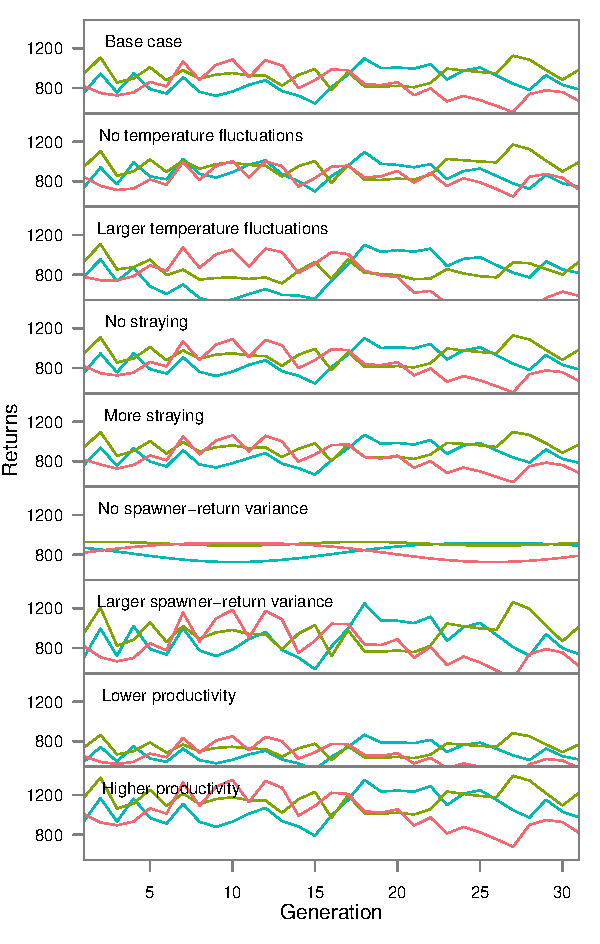
\includegraphics[width=4.0in]{../examples/figure/plot-various-options-ts-3pops.pdf}
\caption{The impact of increasing or decreasing various parameter values in the simulations. The different lines represent different salmon populations. (NEED TO ADD PARAMETER VALUES AND EXPAND THIS SLIGHTLY)}
\label{f:eg-sens}
\end{figure}

\clearpage

\begin{figure}[htbp]
\centering
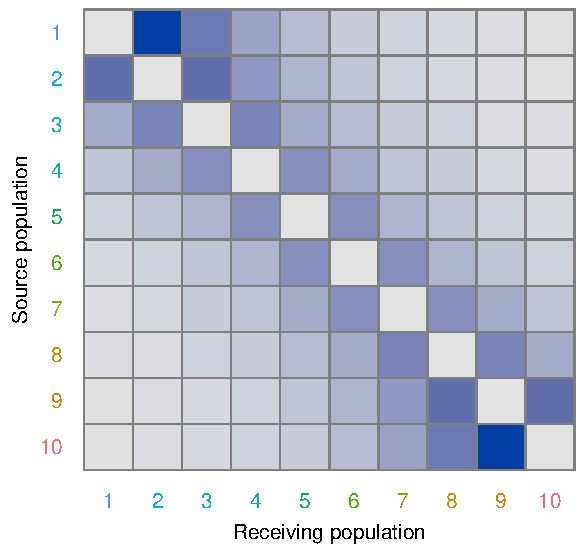
\includegraphics[width=4.0in]{../examples/figure/stray-matrix.pdf}
\caption{An example straying matrix. The rows and columns represent different 
populations (indicated by population number). Dark blue indicates a high rate 
of straying and light blue indicates a low rate of straying. The straying 
matrix is generated through equation \ref{eq:stray}.}
\label{f:stray}
\end{figure}

\clearpage

\begin{figure}[htbp]
\centering
\includegraphics[width=4.5in]{../examples/spatial-arma-sim.pdf}
\caption{Spatial and short-term environmental fluctuations}
\label{f:eg-sp-arma}
\end{figure}

\clearpage

\begin{figure}[htbp]
\centering
\includegraphics[width=4.5in]{../examples/spatial-linear-sim.pdf}
\caption{Spatial and long-term environmental fluctuations}
\label{f:eg-sp-linear}
\end{figure}

\clearpage

\begin{figure}[htbp]
\centering
\includegraphics[width=4.5in]{../examples/n-arma-sim.pdf}
\caption{Number and short-term environmental fluctuations}
\label{f:eg-n-arma}
\end{figure}

\clearpage

\begin{figure}[htbp]
\centering
\includegraphics[width=4.5in]{../examples/n-linear-sim.pdf}
\caption{Number and long-term environmental change}
\label{f:eg-n-linear}
\end{figure}

\clearpage

A placeholder: \citep{schindler2010}

\bibliographystyle{apalike}

\bibliography{jshort,som}


\end{spacing}

\end{document}
